

\section{Redefine stagnation}

\begin{lemma}
\label{lem:unconverge_neq_gb}
A particle won't stop moving when its personal best and global best are not the same, 
which means that 
$ \lim_{k \rightarrow \infty} v(k) \neq 0 $, if $ x^{P} \neq x^{G} $.
\begin{proof} 
There are two existing forces driving the movement of a particle, which are $ \Delta f^{G} $ and $ \Delta f^{P} $.
Thus we have
\begin{equation}
\begin{array}{lcl}
v(k+1) = & \chi ( v(k) + \Delta f^{G} (k) + \Delta f^{P} (k) ) \\
\Delta f^{G} (k) = & \phi^{G} u^{G} (k) (x^{G} - x(k)) \\
\Delta f^{P} (k) = & \phi^{P} u^{P} (k) (x^{P} - x(k)) 
\end{array}
\end{equation}
We can see that when $ \Delta f^{G} + \Delta f^{P} \neq 0 $, $ v(k)  \not \rightarrow 0 $.
When $ x^{P} \neq x^{G} $, $ \forall u^{P}(k), u^{G}(k) \in [0, 1] $, $ \not \exists x(k) $, $ \phi^{G} u^{G} (k) (x^{G} - x(k)) + \phi^{P} u^{G} (k) (x^{P} - x(k)) = 0 $.
It means that there exists no equilibrium due to the random factors $ u^{G} (k) $ and $ u^{P} (k) $. 
\end{proof}
\end{lemma}

The stagnation phenomenon is usually modeled as that the global best and personal best are not updated.
By Lemma \ref{lem:unconverge_neq_gb}, we know that in this case, the particle will never really converge.
However, in most of the cases, the personal best is highly likely to be updated if it is not the same with the global best.

Thus, we define ``stagnation'' as the global best is not updated.
In the topology in Figure \ref{fig:topology3}, the role of the global best is like a leader in the swarm, while all the particles run locally by updating the current positions and the personal best.
We can have Property \ref{prop:stagnation_decompose}.

\begin{property}
\label{prop:stagnation_decompose}
The dynamics of a swarm can be decomposed into a sequence of stagnations.
In each stagnation, the global best is not changed.
In each stagnation, there is a particle not moving, whose global best and personal best are the same.
It works as a leader in a flock structure.
When a new global best is found, the swarm moves into a new stagnation.
The particle that finds the new global best becomes a new leader.
\end{property}

By the topology in Figure \ref{fig:topology3}, we also notice that interactions between the particles are maintained by the update of the global best.
When the global best is not changed, the behaviors of the particles are actually decoupled.
Thus we can have Property \ref{prop:decoupled_particles}.

\begin{property}
\label{prop:decoupled_particles}
In stagnation, every particle only has interaction with the leader in the swarm.
\end{property}

As in Figure \ref{fig:categorize_regions}, the solution space will be divided into three types of regions by the global best and the personal best.
\begin{itemize}
\item $ f(x) > f(x^G) $
Once a particle gets into this region, it updates both global best and personal best. 
It becomes a leader of the swarm.
\item $ f(x^{G}) > f(x) > f(x^{P}) $
Once a particle gets into this region, it updates only the personal best.
The solution space is then re-divided.
\item $ f(x) < f(x^{P}) $
When a particle is in this region, it only moves as a random walk.
\end{itemize}

\begin{figure}
\centering
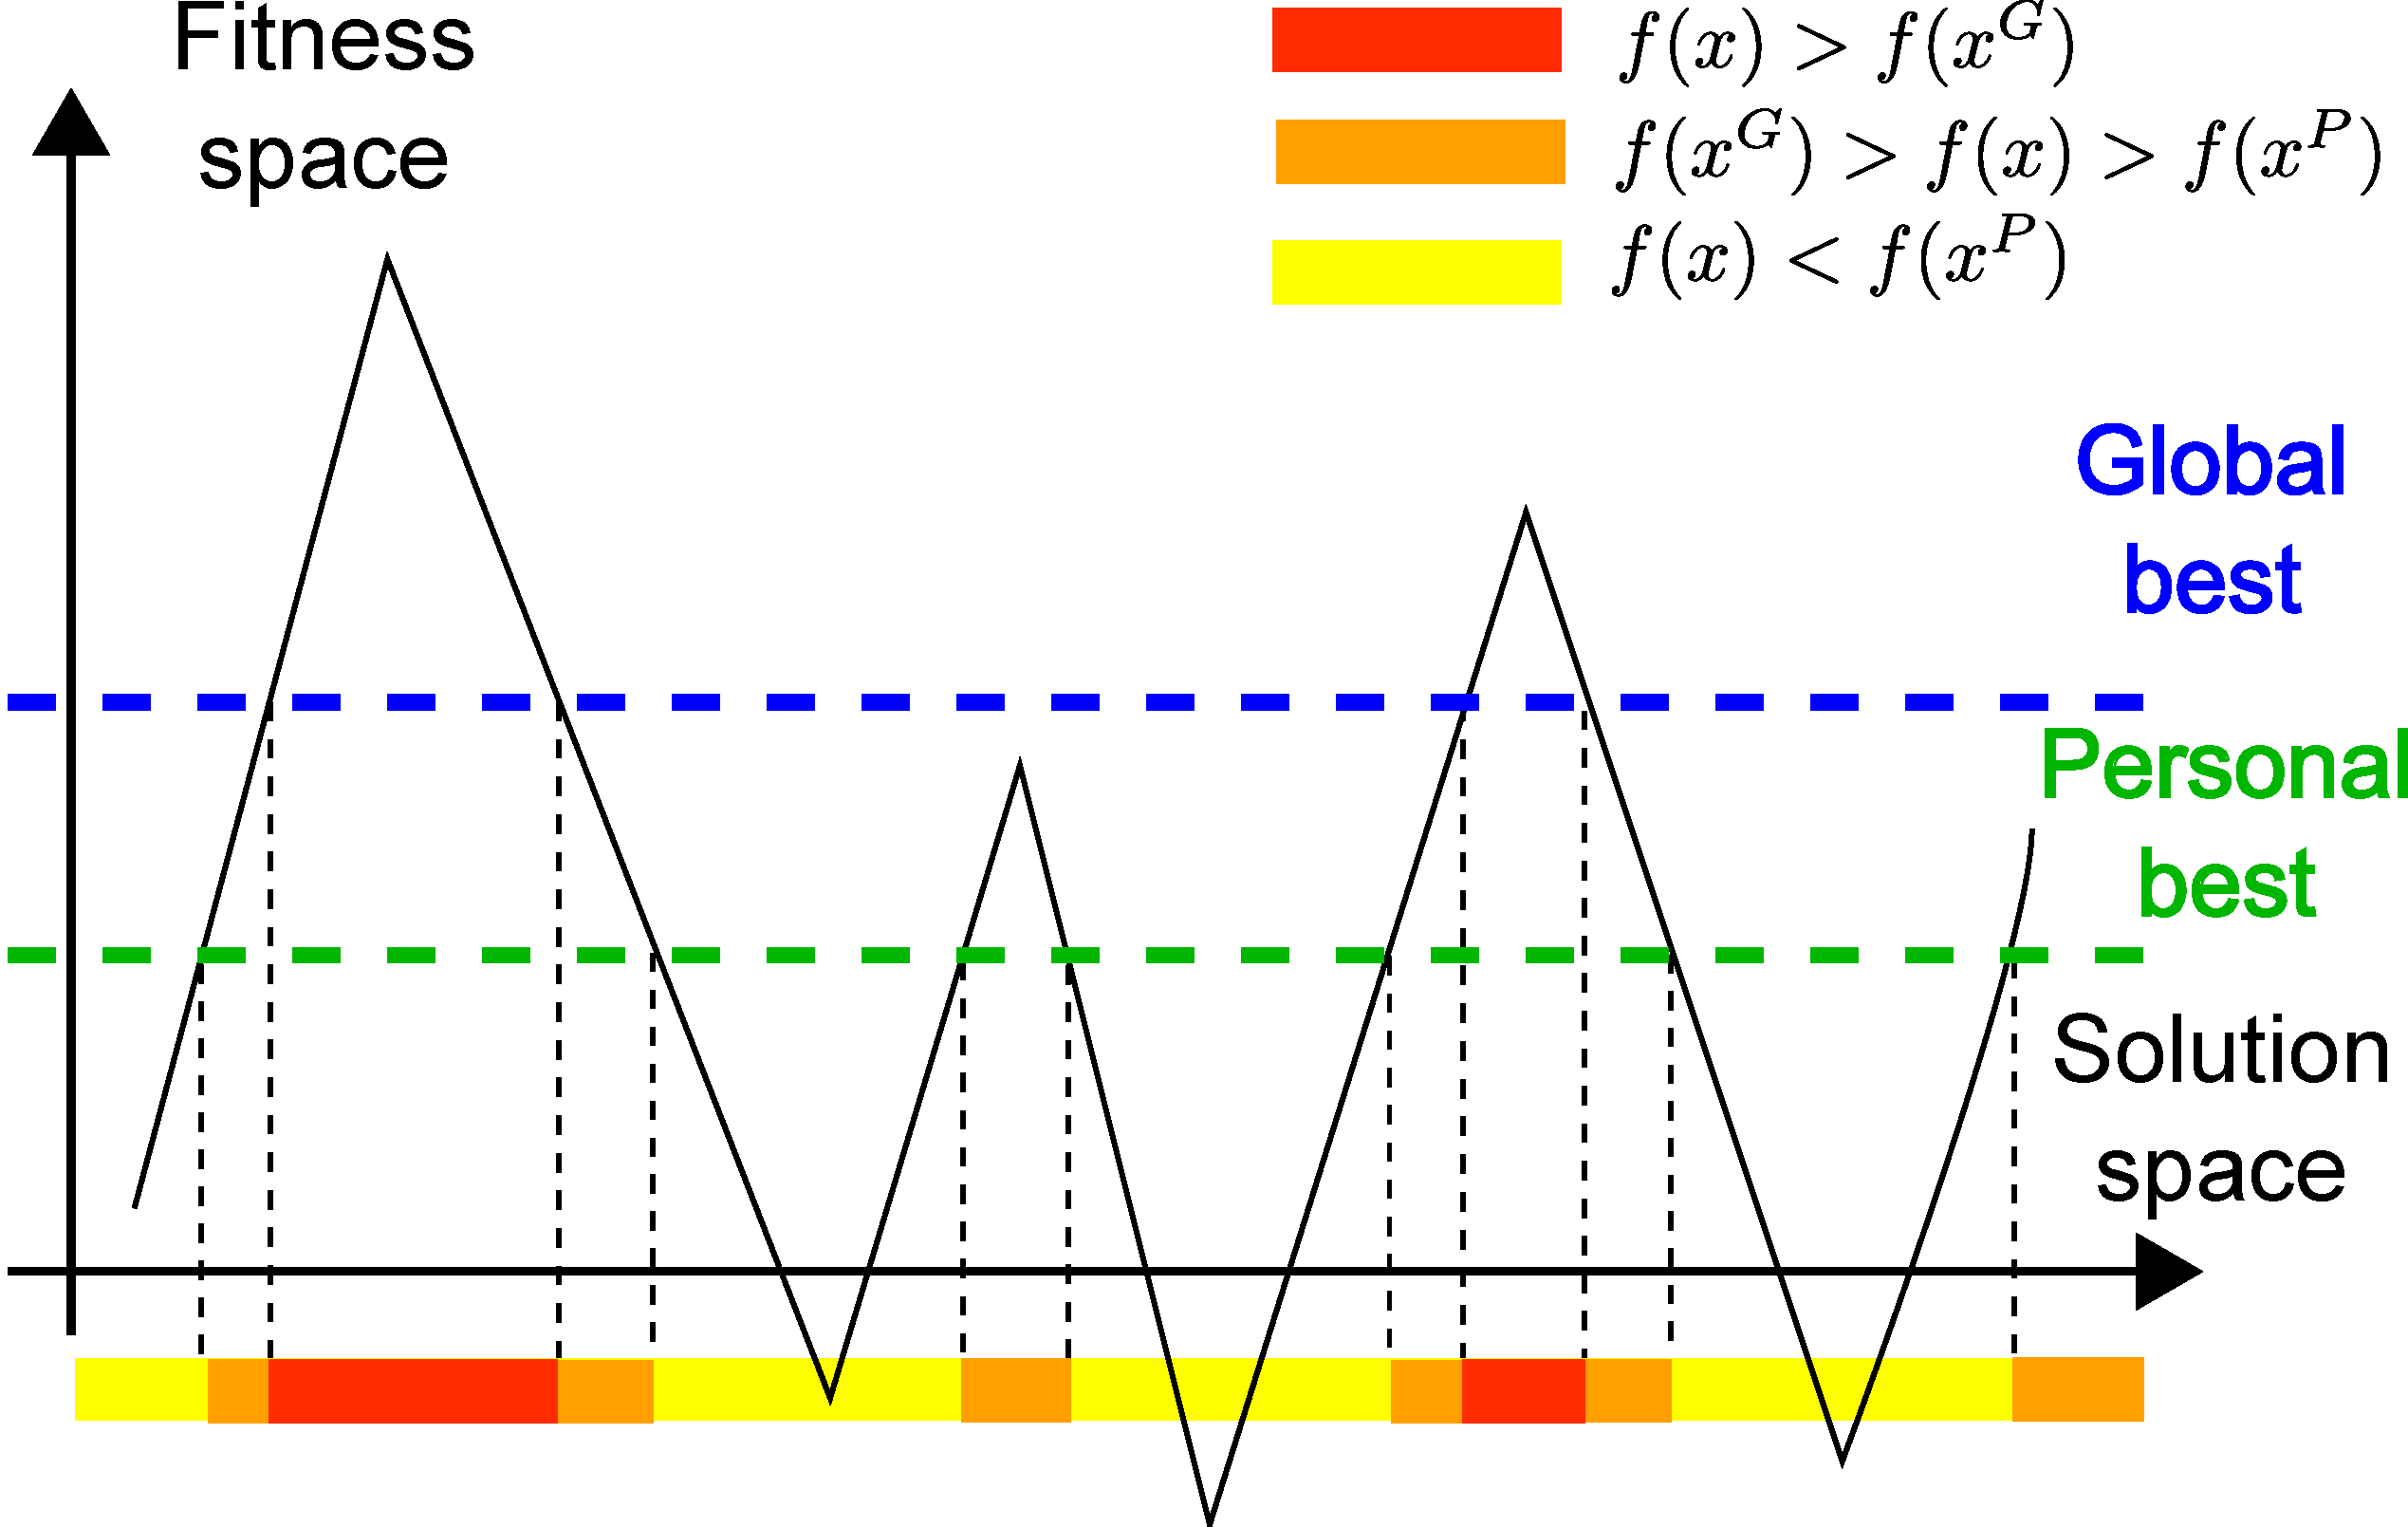
\includegraphics[width=0.7\linewidth]{./categorize_regions}
\caption{How global best and personal best divide the solution space.}
\label{fig:categorize_regions}
\end{figure}


